\section{hoodie}
HOODIE ist eine JavaScript Bibliothek für offlinefähige Webapplikationen, die ein komplettes Backend zur Verfügung stellt. Wird HOODIE für die Entwicklung einer Webanwendung verwendet, muss also lediglich das Frontend implementiert werden. Den Rest erledigt die Bibliothek. Über eine integrierte Programmierschnittstelle kommuniziert die Anwendung mit dem von HOODIE zur Verfügung gestelltem Backend. Über das \gls{API} können unter Anderen BenutzerInnen authentifiziert, Daten gespeichert und synchronisiert werden~\cite{hoodie}.\\
Anhand der Abbildung \ref{fig:hoodie} wird erklärt wie HOODIE funktioniert.
\begin{figure}[H]
  \centering
  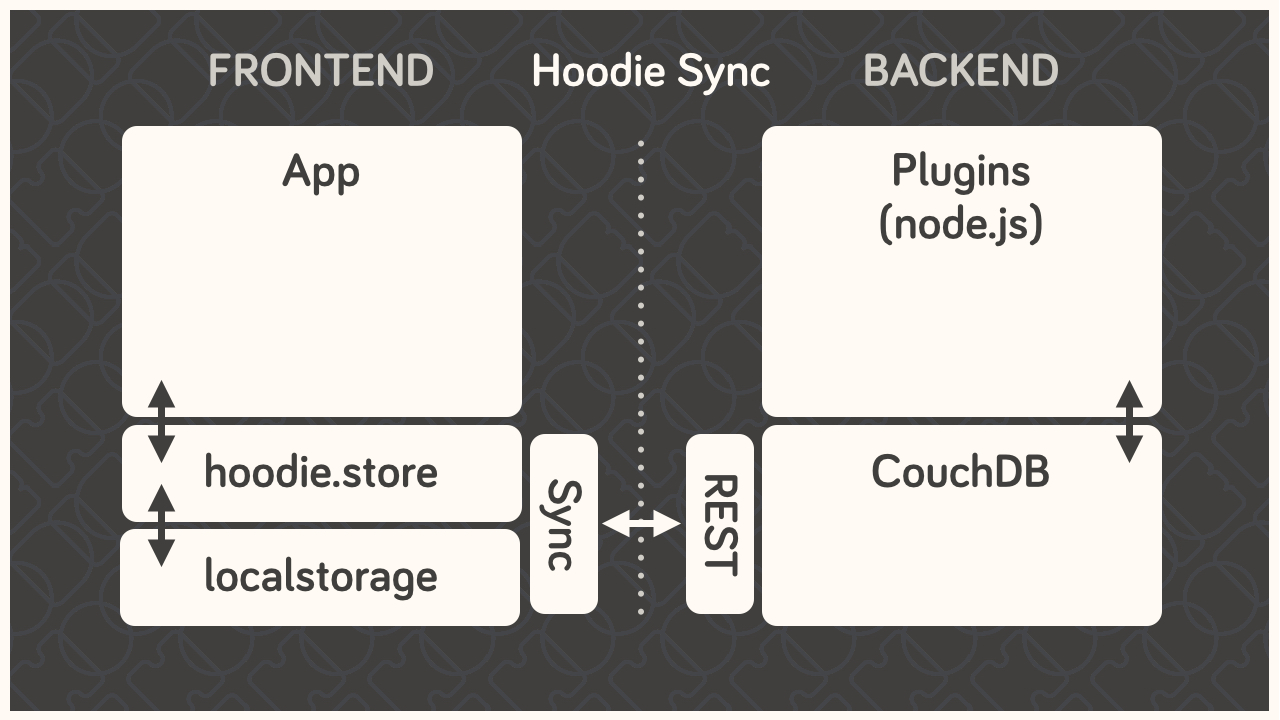
\includegraphics[width=0.8\textwidth]{hoodie}
  \grayRule
  \caption[HOODIE Architektur]{HOODIE Architektur~Quelle:~\cite{hoodie-how}}
  \label{fig:hoodie}
\end{figure}
Im Frontend--Bereicht ist die App zu sehen die über das HOODIE \gls{API} mit dem lokalen Speicher kommuniziert. Die Anwendung spricht niemals direkt mit dem Server oder der Datenbank. Für die lokale Speicherung der Daten benutzt HOODIE intern PouchDB, was wiederum IndexedDB verwendet. Durch das lokale Speichern sind die Daten auch offline verfügbar. Dann werden über eine \gls{REST} Schnittstelle mit einer CouchDB synchronisiert. CouchDB ist eine Datenbank mit der Superkraft des Synchronisierens und in HOODIE haben alle AnwenderInnen ihre eigene private CouchDB. Hinter der Datenbank befindet sich ein kleiner Server der auf die Daten in der CouchDB reagiert, die wiederum die Änderungen an den Client schickt ~\cite{hoodie-how}.
So können NutzerInnen nur auf ihre eigenen Daten zugreifen. Wenn es mehrere Geräte gibt, die mit einem Account assoziiert werden, werden die Änderungen von einem Gerät zuerst auf die serverseitige CouchDB synchronisiert, um dann von dort in die lokalen Datenbanken der anderen Geräte zu gelangen.\\
Dadurch dass das Frontend und das Backend nicht direkt miteinander sprechen, ist die Funktionalität beider Komponenten auch dann gewährleistet, wenn die Verbindung unterbrochen wird.